% Setup
\documentclass[a4 paper, 12pt]{article}

% Title
\title{COSC3000 - REPORT \\ Visualisation}
\author{Teanlouise}
\date{\today}

% Margins
\usepackage{geometry}
\geometry{margin=2cm}

% Images
\usepackage{graphicx}
\usepackage{float}
\usepackage[export]{adjustbox}
\setlength{\intextsep}{5pt plus 2pt minus 2pt}
\usepackage[font=small,skip=5pt]{caption}


% Paragraph
\setlength{\parindent}{2em}
\setlength{\parskip}{1em}

% Text Formatting
\usepackage[utf8]{inputenc}
\usepackage[english]{babel}

% List spacing
\usepackage{enumitem}
\setlist{noitemsep, topsep=0pt}
\setlist[enumerate]{parsep=5pt} 

% Text Color
\usepackage{xcolor}

% Hyperlinks
\usepackage{hyperref}
\hypersetup{
    colorlinks=true,
    linkcolor=black,
    filecolor=black,      
    urlcolor=blue,
}

% Appendix
\usepackage{appendix}

% Include pdf
\usepackage{standalone}
\usepackage{pdfpages}

% Borders
\usepackage{mdframed}




%%%%%%%%%%%%%%%%%%%%%%%%%%%%%%%%%%%%%%%%%%
% DOCUMENT
\begin{document}

% Title
\maketitle

% Table of contents
\pagebreak
\tableofcontents

% Body
\pagebreak
\section{Introduction}
The topic of this project is the Modern Olympics. The games have been a global competition since 1896 with both Summer and Winter sports. The goal is to analyse the patterns of a medal winner depending on their physical characteristics (weight, height, age, sex), home country (athleticism, GDP, population) and the games in which they compete (location). The Olympics are supposed to be a celebration of peace, inclusion and human persistence. It is an opportunity for people to be proud of their country, and be in awe of the feats of athletes. By exploring the above topics it may be possible to determine whether there is a fair representation at the Olympics, and whether the winners are too predictable. If this is the case than the Olympics are no longer serving their purpose.

\section{About the data}
To explore and understand how the Olympics has changed over time, a variety of data was collected from numerous sources. There are three main sources broken up over five datasets. 

    \subsection{Athlete Information}
    The first set of data that needs to be collected relates to the Athlete's information. This includes their physical characteristics (height, weight, age), their role in the Olympics (sport, medal, country) and when they competed (season, year). This information is available for public download on Kaggle under the title '120 years of Olympic history (1896 - 2018)'. This dataset was created by scraping from \url{www.sport-reference.com}. The data is broken down into two files:

        \begin{enumerate}
            \item Athlete and Events - This file contains all of the information recorded about the athlete from all Modern Olympics. The variables of interest are ID, Sex, Age, Height, Weight, NOC, Year, Season and Medal. 
                \begin{figure} [H]
                    \centering
                    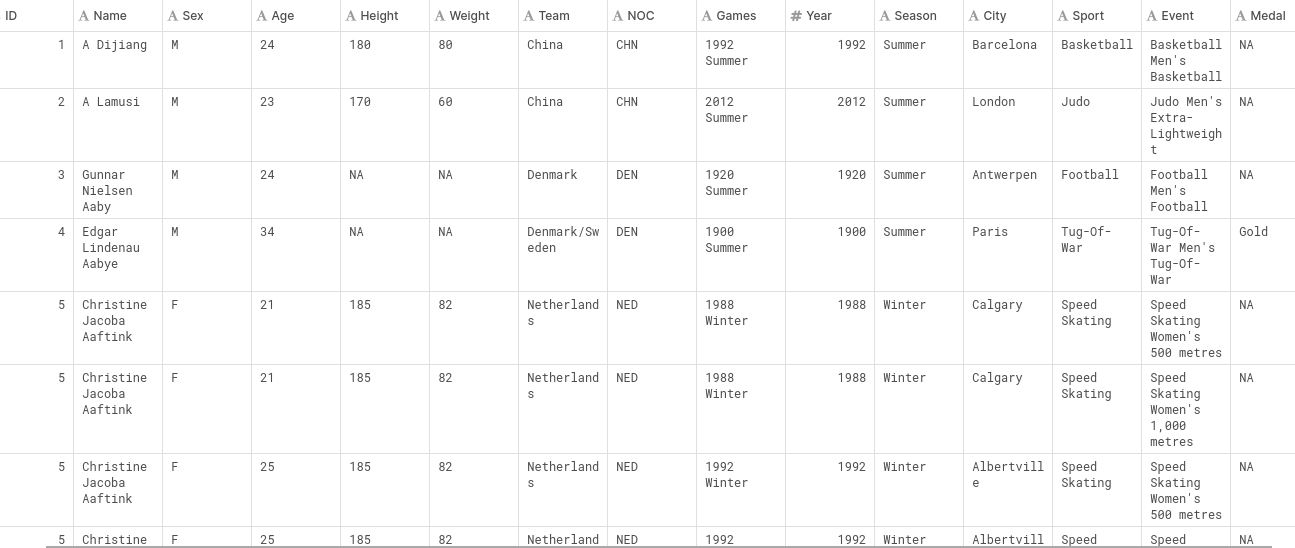
\includegraphics[width=\textwidth, frame]
                        {../images/history_data.png} 
                    \caption{athlete\_events.csv}                  
                \end{figure}            
            \item NOC regions - A list of the countries and their NOC code. It is important to note some countries changed their code in the data. This is noted in Appendix A. 
                \begin{figure}[H]
                    \centering
                    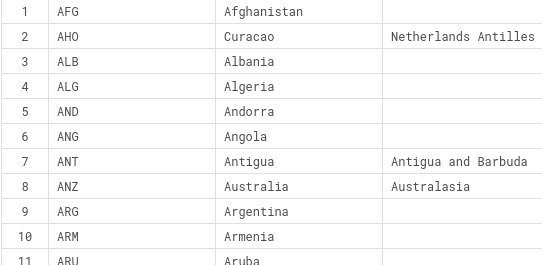
\includegraphics[width=0.6\textwidth, frame]
                    {../images//noc_data.png}   
                    \caption{noc\_regions.csv}                 
            \end{figure}
        \end{enumerate}

    \subsection{Country Information}
    The second set of data relates to the information about each country, including their GDP and population. The most trustworthy source for this data publicly available from World Bank national accounts data, and OECD National Accounts data files. The data is available from 1960 to present, and is accessed as separate files. 
        \begin{enumerate}
            \item GDP - The GDP for all countries, represented in current US\$.
                \begin{figure} [H]
                    \centering
                    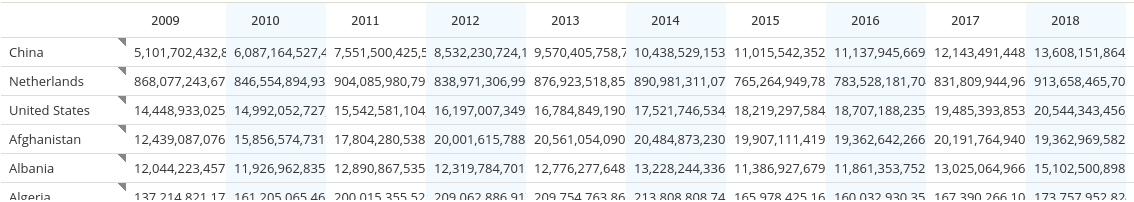
\includegraphics[width=\textwidth, frame]
                        {../images/gdp_data.png}
                        \caption{gdp.csv}                    
                \end{figure}
            \item Population - The total population of all countries.
                \begin{figure} [H]
                    \centering
                    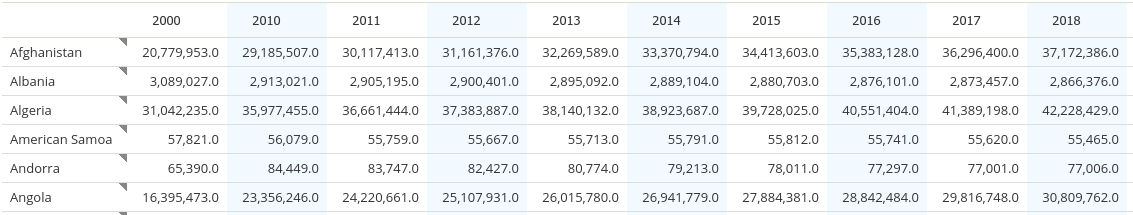
\includegraphics[width=\textwidth, frame]
                        {../images/pop_data.png}      
                        \caption{population.csv} 
                \end{figure} 
        \end{enumerate}

    \subsection{Host Cities}
    The finally set of data is location of each of the games. The 'City' is included as a column in 'athlete\_events.csv', however it is not paired with a country which is needed to compare an athlete's country with where they are competing. This data was not readily available as a data file and so a csv file was manually created from the information found on \url{https://architectureofthegames.net/olympic-host-cities/}. The file contains the year, city, country and season of each Olympic games. 
        \begin{figure} [H]
            \centering
            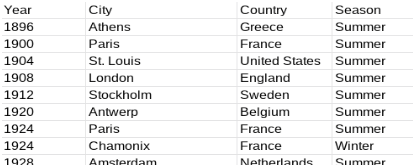
\includegraphics[width=0.6\textwidth, frame]
            {../images/host_data.png}  
            \caption{host\_city.csv}                  
        \end{figure}  

    \subsection{Final Dataset}
    From these files, a new dataset was created using pandas (and article research) to refine the data selection, remove redundancies, combine related variables and update incorrect data to ensure a cleaner dataset for the visualisations. These steps were taken to combine the following five datasets:

        \begin{enumerate}
            \item Remove 'Name', 'Team', 'Games', 'Event', 'Sport' from athlete\_events.csv
                \begin{itemize}
                    \item 'Name' this is not relevant
                    \item 'Team' sometimes contradicts NOC/Country
                    \item 'Games' is duplicate, already split into 'Year' and 'Season'
                    \item 'Event' is not relevant and not consistently
                    \item 'Sport' is not relevant        
                \end{itemize}
            \item Remove Years 1896-1920 from athlete\_events.csv
                \begin{itemize}
                    \item Women didn't compete in 1896
                    \item Winter Games didn't commence until 1924
                \end{itemize}
            \item Make NOC codes consistent for countries that have changed.
                \begin{itemize}
                    \item Russia (RUS): URS (1952-1988), EUN (1992), RUS (1994-2018)
                    \item Taiwan (TPE): ROC (1952-1976), TPE(1984-2018)
                    \item China (CHN): ROC (1924-1948), CHN (1980-2018)
                    \item Germany (GER): GER (1896-2018), EUA (1956-1964), FRG \& GDR (1968-1988)
                    \item Czech Republic (CZE): CZE (1994-2018), TCH (1920-1992), BOH (1900-1912)
                    \item Serbia (SRB): SCG (2004-2006), SRB (1912, 2008-2018), YUG (1920-2002)
                \end{itemize}
            
            \item Add column COUNTRY by matching ‘NOC’ with the same from noc\_regions.csv
            \item Add column HOST COUNTRY by matching ‘country’ with same from host\_city.csv
            \item Add column GDP by matching ‘country’ in gdp.csv
            \item Add column POPULATION by matching ‘country’ in population.csv  
        \end{enumerate}
    
        \begin{figure} [H]
            \centering
            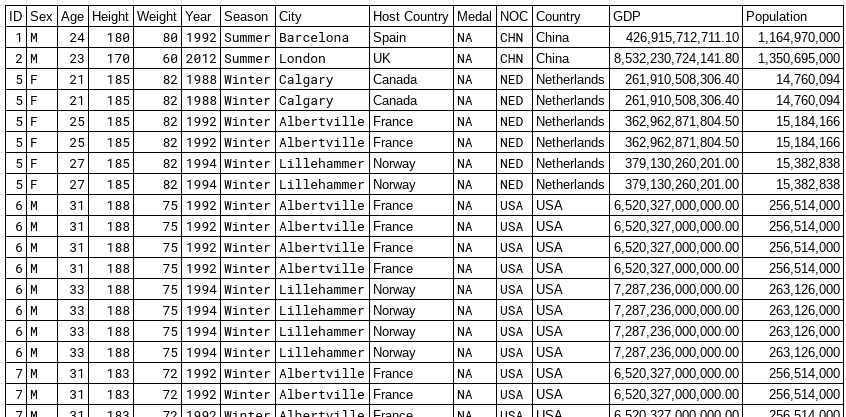
\includegraphics[width=\textwidth, frame]
                {../images/new_data.png}     
            \caption{all\_data.csv}               
        \end{figure} 


\section{Discussion}
The prediction of medal winners will be explored through a number of topics. Each of these will be presented as a comparison between the winter and summer games. Data will be considered from 1924 (when the Winter Olympics were introduced), except for BMI, GDP and population which will be taken from 1960 (when data is collected for majority of points for these variables). The variables ‘NOC’, ‘year’ and ‘season’ are used for all analysis. From current knowledge these are possible visualisations that can be explored:
    \begin{itemize}
        \item The distribution of the number of events and medals [Histogram (\#events, \#medal)]
        \item The change in age for medal and non-medal winners [Turkey box (year v. age)]
        \item The BMI of medal and non-medal winners [q-q plot (medal v. non-medal BMI)]
        \item The proportion of medal winners to number athletes [scatter (\#athletes v. \#medals)]
        \item The proportion of men and women competing [scatter (\#females v. \#males)]
        \item The difference in \% of medals when competing at host [scatter (\% hosting v. visiting)]
        \item The effect of population and GDP on number of medals [multi \- pop, GDP, \#medals]
    \end{itemize}




% Appendix
\pagebreak
\appendix
\addappheadtotoc
\appendixpage
\section{Important notes about the data}
    \begin{enumerate}
        \item athlete\_events.csv - Possible factors that may affect results of each Olympics
            \begin{itemize}
                \item 1924: Winter games commence
                \item 1928: Women now compete in more than 2 sports
                \item 1932: Low attendance due to Great Depression
                \item 1940 \& 1944: Cancelled due to WW2
                \item 1948: Art sports (architecture, literature, music, painting, sculpture) removed
                \item 1952: USSR/Russia starts competing, Republic of China (ROC) discontinued
                \item 1956: Boycotts by 8 nations, including China
                \item 1960: Height and Weight measured consistently from now
                \item 1976: Boycotts by 25 nations (mostly from Africa)
                \item 1980: Boycotts by 66 nations, including US
                \item 2000: Summer Olympics capped at 28 sports, 300 events, 10,000 athletes                
            \end{itemize}

        \item noc\_regions.csv - The following countries are recorded under multiple codes:
            
        \begin{itemize}
                \item Australia: AUS, ANZ (New Zealand, 1908\-1912)
                \item Russia: URS (1952\-1988), EUN (1992), RUS (1994\-2018)
                \item China: ROC (1924\-1948), CHN (1952\-2018), HKG (Hong Kong, 1952\-2018)
                \item Germany: GER (1896\-2018), EUA (1956\-1964), FRG \& GDR (1968\-1988)
                \item Czech Republic: CZE (1994\-2018), TCH (1920\-1992), BOH (1900\-1912)
                \item Serbia: SCG (2004\-2006), SRB (1912, 2008\-2018), YUG (1920\-2002)                    
            \end{itemize}  

    \end{enumerate}
\end{document}